\documentclass[tikz]{standalone}
\usepackage{amsmath}
\definecolor{bg}{HTML}{171D2B}
\definecolor{aksen}{HTML}{F7B538}
\begin{document}
\pagecolor{bg}
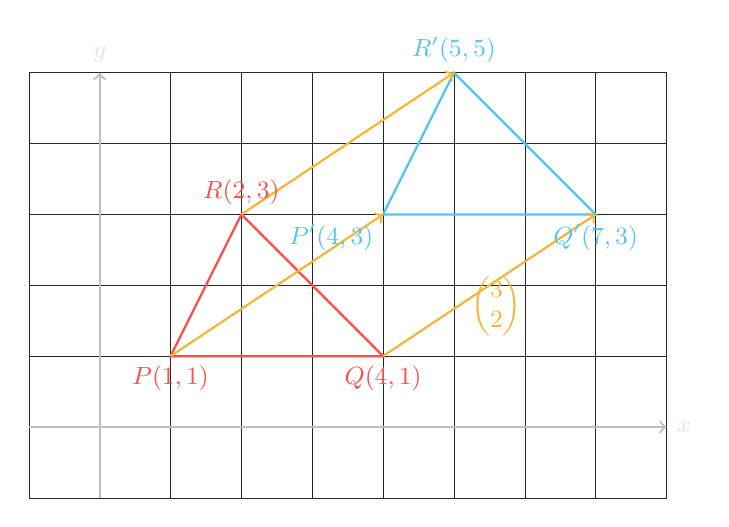
\begin{tikzpicture}[
    scale=0.9,
    axis/.style={->, white!75!black, thick},
    gridline/.style={white!15!black, very thin},
    asal/.style={red!70!white},
    bayang/.style={cyan!70!white},
    panah/.style={->, thick, aksen},
    lbl/.style={white!90!black, font=\small},
  ]
  % grid dan sumbu
  \draw[gridline] (-1,-1) grid (8,5);
  \draw[axis] (-1,0) -- (8,0) node[right, lbl] {$x$};
  \draw[axis] (0,-1) -- (0,5) node[above, lbl] {$y$};

  % segitiga asal (merah)
  \coordinate (P) at (1,1);
  \coordinate (Q) at (4,1);
  \coordinate (R) at (2,3);
  \draw[thick, asal] (P) -- (Q) -- (R) -- cycle;

  % bayangan (biru) = asal + (3,2)
  \coordinate (P') at (4,3);
  \coordinate (Q') at (7,3);
  \coordinate (R') at (5,5);
  \draw[thick, bayang] (P') -- (Q') -- (R') -- cycle;

  % panah translasi di tiap titik
  \foreach \p/\q in {P/P', Q/Q', R/R'} {
    \draw[panah] (\p) -- (\q);
  }

  % label titik
  \node[below, asal, font=\small] at (P) {$P(1,1)$};
  \node[below, asal, font=\small] at (Q) {$Q(4,1)$};
  \node[above, asal, font=\small] at (R) {$R(2,3)$};
  \node[below left, bayang, font=\small] at (P') {$P'(4,3)$};
  \node[below, bayang, font=\small] at (Q') {$Q'(7,3)$};
  \node[above, bayang, font=\small] at (R') {$R'(5,5)$};

  % label vektor
  \node[lbl, font=\small, aksen] at (5.6,1.7) {$\begin{pmatrix}3\\2\end{pmatrix}$};
\end{tikzpicture}
\end{document}
